\documentclass[1p]{elsarticle_modified}
%\bibliographystyle{elsarticle-num}

%\usepackage[colorlinks]{hyperref}
%\usepackage{abbrmath_seonhwa} %\Abb, \Ascr, \Acal ,\Abf, \Afrak
\usepackage{amsfonts}
\usepackage{amssymb}
\usepackage{amsmath}
\usepackage{amsthm}
\usepackage{scalefnt}
\usepackage{amsbsy}
\usepackage{kotex}
\usepackage{caption}
\usepackage{subfig}
\usepackage{color}
\usepackage{graphicx}
\usepackage{xcolor} %% white, black, red, green, blue, cyan, magenta, yellow
\usepackage{float}
\usepackage{setspace}
\usepackage{hyperref}

\usepackage{tikz}
\usetikzlibrary{arrows}

\usepackage{multirow}
\usepackage{array} % fixed length table
\usepackage{hhline}

%%%%%%%%%%%%%%%%%%%%%
\makeatletter
\renewcommand*\env@matrix[1][\arraystretch]{%
	\edef\arraystretch{#1}%
	\hskip -\arraycolsep
	\let\@ifnextchar\new@ifnextchar
	\array{*\c@MaxMatrixCols c}}
\makeatother %https://tex.stackexchange.com/questions/14071/how-can-i-increase-the-line-spacing-in-a-matrix
%%%%%%%%%%%%%%%

\usepackage[normalem]{ulem}

\newcommand{\msout}[1]{\ifmmode\text{\sout{\ensuremath{#1}}}\else\sout{#1}\fi}
%SOURCE: \msout is \stkout macro in https://tex.stackexchange.com/questions/20609/strikeout-in-math-mode

\newcommand{\cancel}[1]{
	\ifmmode
	{\color{red}\msout{#1}}
	\else
	{\color{red}\sout{#1}}
	\fi
}

\newcommand{\add}[1]{
	{\color{blue}\uwave{#1}}
}

\newcommand{\replace}[2]{
	\ifmmode
	{\color{red}\msout{#1}}{\color{blue}\uwave{#2}}
	\else
	{\color{red}\sout{#1}}{\color{blue}\uwave{#2}}
	\fi
}

\newcommand{\Sol}{\mathcal{S}} %segment
\newcommand{\D}{D} %diagram
\newcommand{\A}{\mathcal{A}} %arc


%%%%%%%%%%%%%%%%%%%%%%%%%%%%%5 test

\def\sl{\operatorname{\textup{SL}}(2,\Cbb)}
\def\psl{\operatorname{\textup{PSL}}(2,\Cbb)}
\def\quan{\mkern 1mu \triangleright \mkern 1mu}

\theoremstyle{definition}
\newtheorem{thm}{Theorem}[section]
\newtheorem{prop}[thm]{Proposition}
\newtheorem{lem}[thm]{Lemma}
\newtheorem{ques}[thm]{Question}
\newtheorem{cor}[thm]{Corollary}
\newtheorem{defn}[thm]{Definition}
\newtheorem{exam}[thm]{Example}
\newtheorem{rmk}[thm]{Remark}
\newtheorem{alg}[thm]{Algorithm}

\newcommand{\I}{\sqrt{-1}}
\begin{document}

%\begin{frontmatter}
%
%\title{Boundary parabolic representations of knots up to 8 crossings}
%
%%% Group authors per affiliation:
%\author{Yunhi Cho} 
%\address{Department of Mathematics, University of Seoul, Seoul, Korea}
%\ead{yhcho@uos.ac.kr}
%
%
%\author{Seonhwa Kim} %\fnref{s_kim}}
%\address{Center for Geometry and Physics, Institute for Basic Science, Pohang, 37673, Korea}
%\ead{ryeona17@ibs.re.kr}
%
%\author{Hyuk Kim}
%\address{Department of Mathematical Sciences, Seoul National University, Seoul 08826, Korea}
%\ead{hyukkim@snu.ac.kr}
%
%\author{Seokbeom Yoon}
%\address{Department of Mathematical Sciences, Seoul National University, Seoul, 08826,  Korea}
%\ead{sbyoon15@snu.ac.kr}
%
%\begin{abstract}
%We find all boundary parabolic representation of knots up to 8 crossings.
%
%\end{abstract}
%\begin{keyword}
%    \MSC[2010] 57M25 
%\end{keyword}
%
%\end{frontmatter}

%\linenumbers
%\tableofcontents
%
\newcommand\colored[1]{\textcolor{white}{\rule[-0.35ex]{0.8em}{1.4ex}}\kern-0.8em\color{red} #1}%
%\newcommand\colored[1]{\textcolor{white}{ #1}\kern-2.17ex	\textcolor{white}{ #1}\kern-1.81ex	\textcolor{white}{ #1}\kern-2.15ex\color{red}#1	}

{\Large $\underline{12n_{0535}~(K12n_{0535})}$}

\setlength{\tabcolsep}{10pt}
\renewcommand{\arraystretch}{1.6}
\vspace{1cm}\begin{tabular}{m{100pt}>{\centering\arraybackslash}m{274pt}}
\multirow{5}{120pt}{
	\centering
	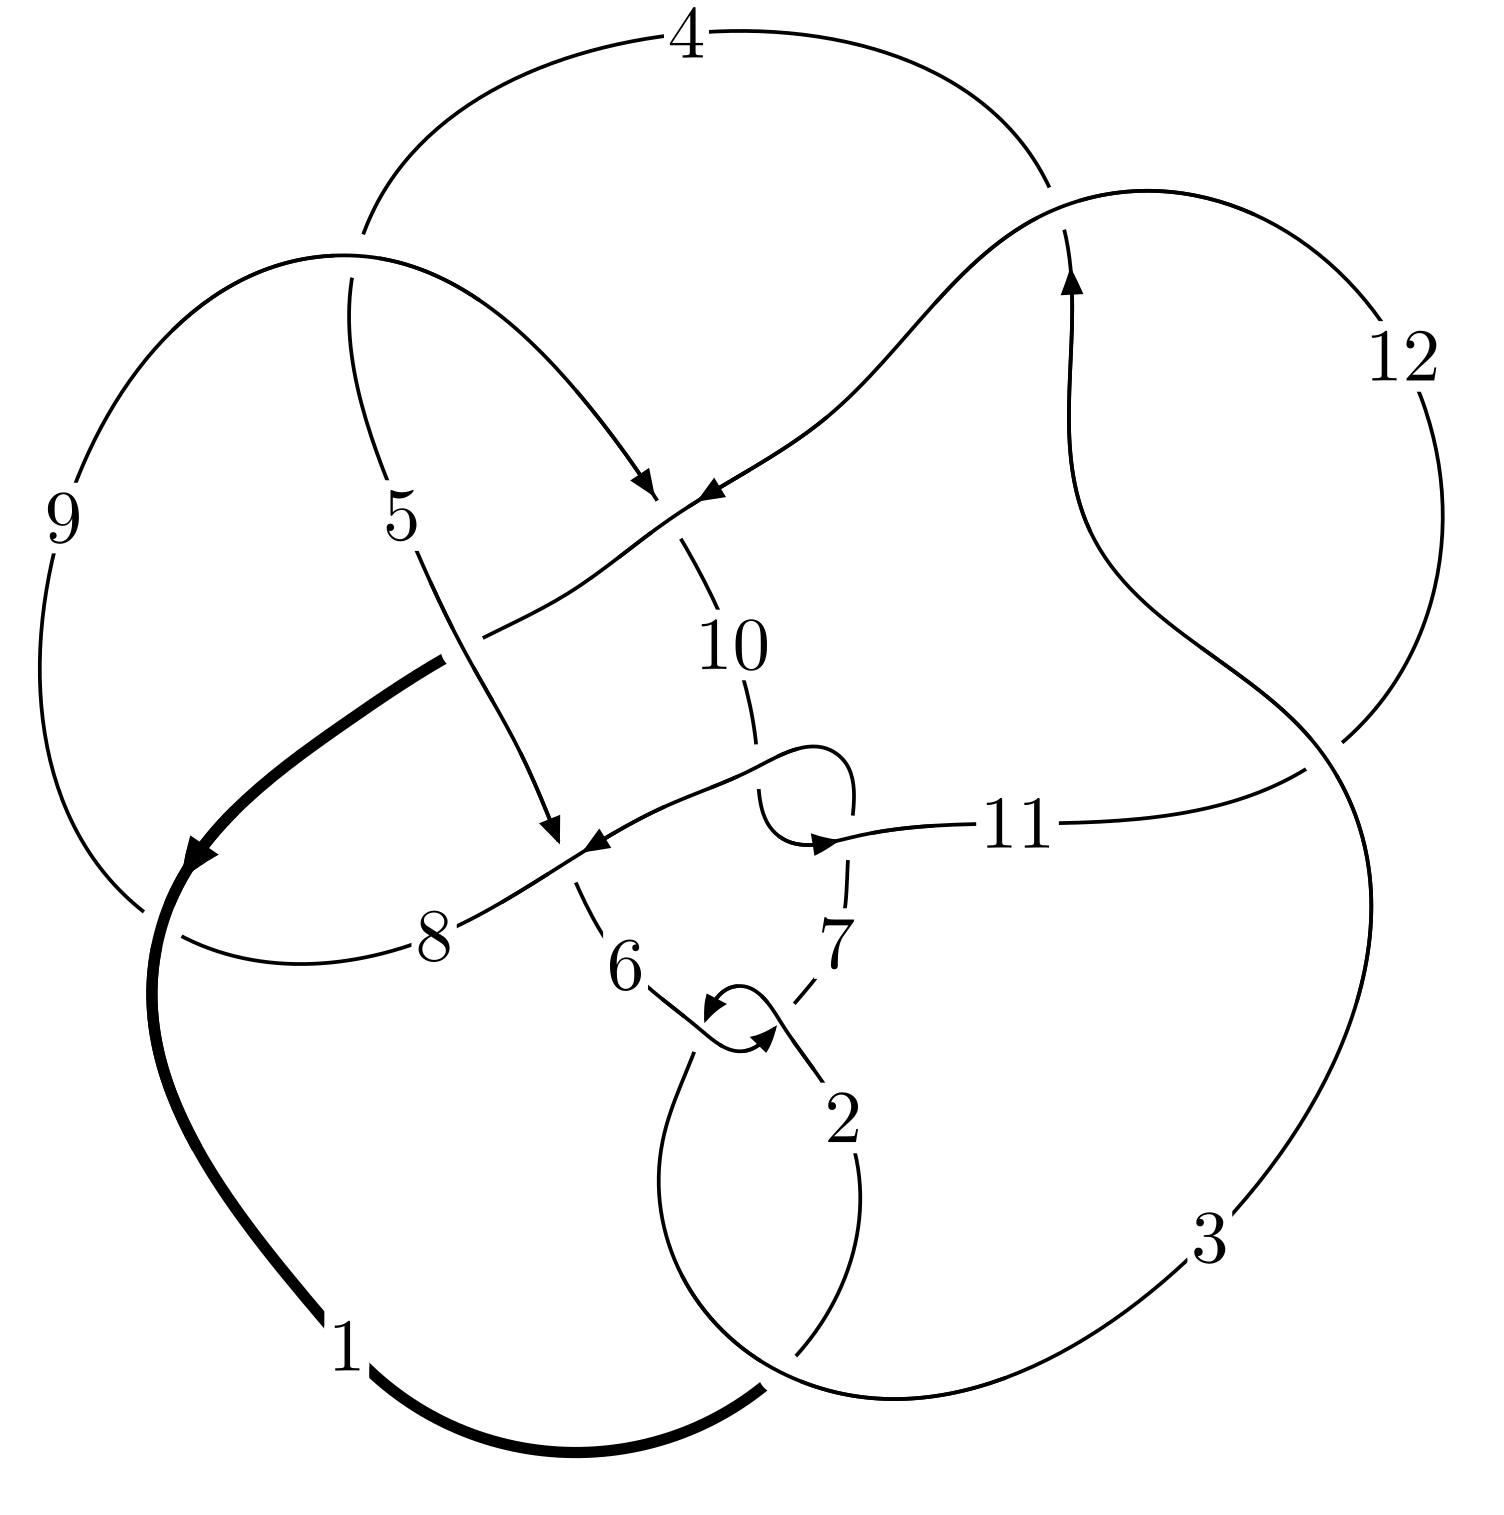
\includegraphics[width=112pt]{../../../GIT/diagram.site/Diagrams/png/2624_12n_0535.png}\\
\ \ \ A knot diagram\footnotemark}&
\allowdisplaybreaks
\textbf{Linearized knot diagam} \\
\cline{2-2}
 &
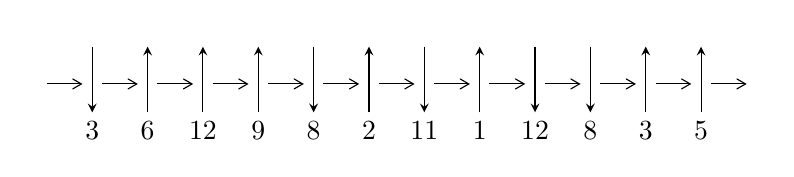
\begin{tikzpicture}[x=20pt, y=17pt]
	% nodes
	\node (C0) at (0, 0) {};
	\node (C1) at (1, 0) {};
	\node (C1U) at (1, +1) {};
	\node (C1D) at (1, -1) {3};

	\node (C2) at (2, 0) {};
	\node (C2U) at (2, +1) {};
	\node (C2D) at (2, -1) {6};

	\node (C3) at (3, 0) {};
	\node (C3U) at (3, +1) {};
	\node (C3D) at (3, -1) {12};

	\node (C4) at (4, 0) {};
	\node (C4U) at (4, +1) {};
	\node (C4D) at (4, -1) {9};

	\node (C5) at (5, 0) {};
	\node (C5U) at (5, +1) {};
	\node (C5D) at (5, -1) {8};

	\node (C6) at (6, 0) {};
	\node (C6U) at (6, +1) {};
	\node (C6D) at (6, -1) {2};

	\node (C7) at (7, 0) {};
	\node (C7U) at (7, +1) {};
	\node (C7D) at (7, -1) {11};

	\node (C8) at (8, 0) {};
	\node (C8U) at (8, +1) {};
	\node (C8D) at (8, -1) {1};

	\node (C9) at (9, 0) {};
	\node (C9U) at (9, +1) {};
	\node (C9D) at (9, -1) {12};

	\node (C10) at (10, 0) {};
	\node (C10U) at (10, +1) {};
	\node (C10D) at (10, -1) {8};

	\node (C11) at (11, 0) {};
	\node (C11U) at (11, +1) {};
	\node (C11D) at (11, -1) {3};

	\node (C12) at (12, 0) {};
	\node (C12U) at (12, +1) {};
	\node (C12D) at (12, -1) {5};
	\node (C13) at (13, 0) {};

	% arrows
	\draw[->,>={angle 60}]
	(C0) edge (C1) (C1) edge (C2) (C2) edge (C3) (C3) edge (C4) (C4) edge (C5) (C5) edge (C6) (C6) edge (C7) (C7) edge (C8) (C8) edge (C9) (C9) edge (C10) (C10) edge (C11) (C11) edge (C12) (C12) edge (C13) ;	\draw[->,>=stealth]
	(C1U) edge (C1D) (C2D) edge (C2U) (C3D) edge (C3U) (C4D) edge (C4U) (C5U) edge (C5D) (C6D) edge (C6U) (C7U) edge (C7D) (C8D) edge (C8U) (C9U) edge (C9D) (C10U) edge (C10D) (C11D) edge (C11U) (C12D) edge (C12U) ;
	\end{tikzpicture} \\
\hhline{~~} \\& 
\textbf{Solving Sequence} \\ \cline{2-2} 
 &
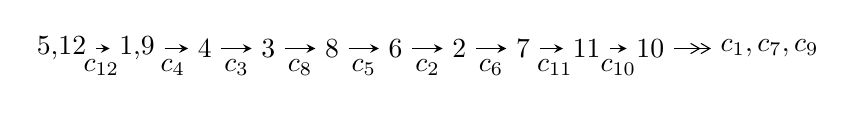
\begin{tikzpicture}[x=23pt, y=7pt]
	% node
	\node (A0) at (-1/8, 0) {5,12};
	\node (A1) at (17/16, 0) {1,9};
	\node (A2) at (17/8, 0) {4};
	\node (A3) at (25/8, 0) {3};
	\node (A4) at (33/8, 0) {8};
	\node (A5) at (41/8, 0) {6};
	\node (A6) at (49/8, 0) {2};
	\node (A7) at (57/8, 0) {7};
	\node (A8) at (65/8, 0) {11};
	\node (A9) at (73/8, 0) {10};
	\node (C1) at (1/2, -1) {$c_{12}$};
	\node (C2) at (13/8, -1) {$c_{4}$};
	\node (C3) at (21/8, -1) {$c_{3}$};
	\node (C4) at (29/8, -1) {$c_{8}$};
	\node (C5) at (37/8, -1) {$c_{5}$};
	\node (C6) at (45/8, -1) {$c_{2}$};
	\node (C7) at (53/8, -1) {$c_{6}$};
	\node (C8) at (61/8, -1) {$c_{11}$};
	\node (C9) at (69/8, -1) {$c_{10}$};
	\node (A10) at (11, 0) {$c_{1},c_{7},c_{9}$};

	% edge
	\draw[->,>=stealth]	
	(A0) edge (A1) (A1) edge (A2) (A2) edge (A3) (A3) edge (A4) (A4) edge (A5) (A5) edge (A6) (A6) edge (A7) (A7) edge (A8) (A8) edge (A9) ;
	\draw[->>,>={angle 60}]	
	(A9) edge (A10);
\end{tikzpicture} \\ 

\end{tabular} \\

\footnotetext{
The image of knot diagram is generated by the software ``\textbf{Draw programme}" developed by Andrew Bartholomew(\url{http://www.layer8.co.uk/maths/draw/index.htm\#Running-draw}), where we modified some parts for our purpose(\url{https://github.com/CATsTAILs/LinksPainter}).
}\phantom \\ \newline 
\centering \textbf{Ideals for irreducible components\footnotemark of $X_{\text{par}}$} 
 
\begin{align*}
I^u_{1}&=\langle 
-34964567 u^{18}-147929889 u^{17}+\cdots+84548050 b-17321241,\\
\phantom{I^u_{1}}&\phantom{= \langle  }-36305359 u^{18}-171870803 u^{17}+\cdots+84548050 a-72540507,\;u^{19}+4 u^{18}+\cdots-3 u^3+1\rangle \\
I^u_{2}&=\langle 
u^5- u^4+2 u^2+b- a+1,\\
\phantom{I^u_{2}}&\phantom{= \langle  }u^6 a-2 u^5 a- u^6+u^4 a+u^5+2 u^3 a- u^4-2 u^2 a-2 u^3+a^2+a u+u^2- a-3 u-1,\\
\phantom{I^u_{2}}&\phantom{= \langle  }u^7-2 u^6+2 u^5+u^4-2 u^3+3 u^2-2 u+1\rangle \\
I^u_{3}&=\langle 
u^3+2 u^2+b+3 u+2,\;- u^3-3 u^2+a-5 u-2,\;u^4+3 u^3+5 u^2+3 u+1\rangle \\
I^u_{4}&=\langle 
- u^5+u^4+b- a-2 u+1,\;u^5 a+a^2+2 a u+u^2,\;u^6- u^5+u^4+2 u^2- u+1\rangle \\
\\
\end{align*}
\raggedright * 4 irreducible components of $\dim_{\mathbb{C}}=0$, with total 49 representations.\\
\footnotetext{All coefficients of polynomials are rational numbers. But the coefficients are sometimes approximated in decimal forms when there is not enough margin.}
\newpage
\renewcommand{\arraystretch}{1}
\centering \section*{I. $I^u_{1}= \langle -3.50\times10^{7} u^{18}-1.48\times10^{8} u^{17}+\cdots+8.45\times10^{7} b-1.73\times10^{7},\;-3.63\times10^{7} u^{18}-1.72\times10^{8} u^{17}+\cdots+8.45\times10^{7} a-7.25\times10^{7},\;u^{19}+4 u^{18}+\cdots-3 u^3+1 \rangle$}
\flushleft \textbf{(i) Arc colorings}\\
\begin{tabular}{m{7pt} m{180pt} m{7pt} m{180pt} }
\flushright $a_{5}=$&$\begin{pmatrix}0\\u\end{pmatrix}$ \\
\flushright $a_{12}=$&$\begin{pmatrix}1\\0\end{pmatrix}$ \\
\flushright $a_{1}=$&$\begin{pmatrix}1\\- u^2\end{pmatrix}$ \\
\flushright $a_{9}=$&$\begin{pmatrix}0.429405 u^{18}+2.03282 u^{17}+\cdots-0.972166 u+0.857980\\0.413547 u^{18}+1.74965 u^{17}+\cdots+0.520629 u+0.204869\end{pmatrix}$ \\
\flushright $a_{4}=$&$\begin{pmatrix}-0.658072 u^{18}-2.36766 u^{17}+\cdots-0.942839 u+0.860317\\-0.0707958 u^{18}+0.0522380 u^{17}+\cdots+0.273040 u+0.587276\end{pmatrix}$ \\
\flushright $a_{3}=$&$\begin{pmatrix}-0.587276 u^{18}-2.41990 u^{17}+\cdots-1.21588 u+0.273040\\-0.0707958 u^{18}+0.0522380 u^{17}+\cdots+0.273040 u+0.587276\end{pmatrix}$ \\
\flushright $a_{8}=$&$\begin{pmatrix}0.0380189 u^{18}+0.291456 u^{17}+\cdots-1.06339 u+0.968309\\0.355477 u^{18}+1.40522 u^{17}+\cdots+0.129243 u+0.0290509\end{pmatrix}$ \\
\flushright $a_{6}=$&$\begin{pmatrix}-0.500327 u^{18}-2.21013 u^{17}+\cdots-0.556008 u+0.0492471\\-0.402635 u^{18}-1.32006 u^{17}+\cdots+0.181729 u+0.279600\end{pmatrix}$ \\
\flushright $a_{2}=$&$\begin{pmatrix}-0.473557 u^{18}-1.49737 u^{17}+\cdots-2.34644 u+1.18683\\0.396856 u^{18}+1.98083 u^{17}+\cdots+0.186827 u+0.473557\end{pmatrix}$ \\
\flushright $a_{7}=$&$\begin{pmatrix}0.761277 u^{18}+3.01695 u^{17}+\cdots-0.400542 u+0.304195\\-0.280164 u^{18}-1.43418 u^{17}+\cdots+1.18128 u-0.688967\end{pmatrix}$ \\
\flushright $a_{11}=$&$\begin{pmatrix}-0.484468 u^{18}-1.92696 u^{17}+\cdots-2.04880 u+0.702358\\0.0109112 u^{18}+0.429590 u^{17}+\cdots-0.297642 u+0.484468\end{pmatrix}$ \\
\flushright $a_{10}=$&$\begin{pmatrix}0.0158583 u^{18}+0.283163 u^{17}+\cdots-1.49279 u+0.653111\\0.413547 u^{18}+1.74965 u^{17}+\cdots+0.520629 u+0.204869\end{pmatrix}$\\&\end{tabular}
\flushleft \textbf{(ii) Obstruction class $= -1$}\\~\\
\flushleft \textbf{(iii) Cusp Shapes $= \frac{20137897}{8454805} u^{18}+\frac{69147964}{8454805} u^{17}+\cdots+\frac{1296527}{8454805} u+\frac{31835641}{8454805}$}\\~\\
\newpage\renewcommand{\arraystretch}{1}
\flushleft \textbf{(iv) u-Polynomials at the component}\newline \\
\begin{tabular}{m{50pt}|m{274pt}}
Crossings & \hspace{64pt}u-Polynomials at each crossing \\
\hline $$\begin{aligned}c_{1}\end{aligned}$$&$\begin{aligned}
&u^{19}+14 u^{18}+\cdots-28 u-4
\end{aligned}$\\
\hline $$\begin{aligned}c_{2},c_{4},c_{6}\end{aligned}$$&$\begin{aligned}
&u^{19}+7 u^{17}+\cdots-2 u-2
\end{aligned}$\\
\hline $$\begin{aligned}c_{3},c_{11}\end{aligned}$$&$\begin{aligned}
&u^{19}+2 u^{18}+\cdots-11 u-1
\end{aligned}$\\
\hline $$\begin{aligned}c_{5},c_{7},c_{10}\end{aligned}$$&$\begin{aligned}
&u^{19}-2 u^{18}+\cdots+2 u-1
\end{aligned}$\\
\hline $$\begin{aligned}c_{8}\end{aligned}$$&$\begin{aligned}
&u^{19}- u^{18}+\cdots-25 u-25
\end{aligned}$\\
\hline $$\begin{aligned}c_{9}\end{aligned}$$&$\begin{aligned}
&u^{19}-3 u^{18}+\cdots+46 u-11
\end{aligned}$\\
\hline $$\begin{aligned}c_{12}\end{aligned}$$&$\begin{aligned}
&u^{19}-4 u^{18}+\cdots-3 u^3-1
\end{aligned}$\\
\hline
\end{tabular}\\~\\
\newpage\renewcommand{\arraystretch}{1}
\flushleft \textbf{(v) Riley Polynomials at the component}\newline \\
\begin{tabular}{m{50pt}|m{274pt}}
Crossings & \hspace{64pt}Riley Polynomials at each crossing \\
\hline $$\begin{aligned}c_{1}\end{aligned}$$&$\begin{aligned}
&y^{19}+26 y^{18}+\cdots-16 y-16
\end{aligned}$\\
\hline $$\begin{aligned}c_{2},c_{4},c_{6}\end{aligned}$$&$\begin{aligned}
&y^{19}+14 y^{18}+\cdots-28 y-4
\end{aligned}$\\
\hline $$\begin{aligned}c_{3},c_{11}\end{aligned}$$&$\begin{aligned}
&y^{19}-32 y^{18}+\cdots+y-1
\end{aligned}$\\
\hline $$\begin{aligned}c_{5},c_{7},c_{10}\end{aligned}$$&$\begin{aligned}
&y^{19}+18 y^{18}+\cdots+44 y-1
\end{aligned}$\\
\hline $$\begin{aligned}c_{8}\end{aligned}$$&$\begin{aligned}
&y^{19}+3 y^{18}+\cdots-1125 y-625
\end{aligned}$\\
\hline $$\begin{aligned}c_{9}\end{aligned}$$&$\begin{aligned}
&y^{19}-23 y^{18}+\cdots+3194 y-121
\end{aligned}$\\
\hline $$\begin{aligned}c_{12}\end{aligned}$$&$\begin{aligned}
&y^{19}-2 y^{18}+\cdots+12 y^2-1
\end{aligned}$\\
\hline
\end{tabular}\\~\\
\newpage\flushleft \textbf{(vi) Complex Volumes and Cusp Shapes}
$$\begin{array}{c|c|c}  
\text{Solutions to }I^u_{1}& \I (\text{vol} + \sqrt{-1}CS) & \text{Cusp shape}\\
 \hline 
\begin{aligned}
u &= \phantom{-}0.821475 + 0.594834 I \\
a &= \phantom{-}1.075950 + 0.336378 I \\
b &= \phantom{-}1.334340 + 0.079123 I\end{aligned}
 & \phantom{-}1.42522 + 6.81402 I & \phantom{-}5.23193 - 9.88797 I \\ \hline\begin{aligned}
u &= \phantom{-}0.821475 - 0.594834 I \\
a &= \phantom{-}1.075950 - 0.336378 I \\
b &= \phantom{-}1.334340 - 0.079123 I\end{aligned}
 & \phantom{-}1.42522 - 6.81402 I & \phantom{-}5.23193 + 9.88797 I \\ \hline\begin{aligned}
u &= -1.173600 + 0.155605 I \\
a &= -0.125477 - 0.508306 I \\
b &= \phantom{-}0.471294 - 0.636829 I\end{aligned}
 & \phantom{-}4.32774 + 1.07425 I & \phantom{-}4.82406 - 6.05931 I \\ \hline\begin{aligned}
u &= -1.173600 - 0.155605 I \\
a &= -0.125477 + 0.508306 I \\
b &= \phantom{-}0.471294 + 0.636829 I\end{aligned}
 & \phantom{-}4.32774 - 1.07425 I & \phantom{-}4.82406 + 6.05931 I \\ \hline\begin{aligned}
u &= \phantom{-}0.279280 + 0.633920 I \\
a &= -0.361697 - 0.610800 I \\
b &= -0.662543 + 0.872189 I\end{aligned}
 & -1.90560 + 1.10773 I & -3.54412 - 5.69242 I \\ \hline\begin{aligned}
u &= \phantom{-}0.279280 - 0.633920 I \\
a &= -0.361697 + 0.610800 I \\
b &= -0.662543 - 0.872189 I\end{aligned}
 & -1.90560 - 1.10773 I & -3.54412 + 5.69242 I \\ \hline\begin{aligned}
u &= -0.612161\phantom{ +0.000000I} \\
a &= \phantom{-}0.732439\phantom{ +0.000000I} \\
b &= \phantom{-}0.209228\phantom{ +0.000000I}\end{aligned}
 & \phantom{-}0.849367\phantom{ +0.000000I} & \phantom{-}11.9240\phantom{ +0.000000I} \\ \hline\begin{aligned}
u &= \phantom{-}0.494731 + 0.181504 I \\
a &= -0.30870 + 2.20346 I \\
b &= -0.343936 + 0.280922 I\end{aligned}
 & \phantom{-}0.84702 - 3.36304 I & \phantom{-}2.65369 + 2.27076 I \\ \hline\begin{aligned}
u &= \phantom{-}0.494731 - 0.181504 I \\
a &= -0.30870 - 2.20346 I \\
b &= -0.343936 - 0.280922 I\end{aligned}
 & \phantom{-}0.84702 + 3.36304 I & \phantom{-}2.65369 - 2.27076 I \\ \hline\begin{aligned}
u &= -1.04681 + 1.06903 I \\
a &= \phantom{-}1.189010 - 0.129598 I \\
b &= \phantom{-}2.18978 + 1.06580 I\end{aligned}
 & \phantom{-}12.2196 - 13.0819 I & \phantom{-}3.46696 + 5.71029 I\\
 \hline 
 \end{array}$$\newpage$$\begin{array}{c|c|c}  
\text{Solutions to }I^u_{1}& \I (\text{vol} + \sqrt{-1}CS) & \text{Cusp shape}\\
 \hline 
\begin{aligned}
u &= -1.04681 - 1.06903 I \\
a &= \phantom{-}1.189010 + 0.129598 I \\
b &= \phantom{-}2.18978 - 1.06580 I\end{aligned}
 & \phantom{-}12.2196 + 13.0819 I & \phantom{-}3.46696 - 5.71029 I \\ \hline\begin{aligned}
u &= -0.135208 + 0.466592 I \\
a &= \phantom{-}2.29915 - 0.00071 I \\
b &= \phantom{-}0.675260 + 1.111080 I\end{aligned}
 & \phantom{-}0.56206 - 3.63168 I & \phantom{-}1.44719 + 4.79816 I \\ \hline\begin{aligned}
u &= -0.135208 - 0.466592 I \\
a &= \phantom{-}2.29915 + 0.00071 I \\
b &= \phantom{-}0.675260 - 1.111080 I\end{aligned}
 & \phantom{-}0.56206 + 3.63168 I & \phantom{-}1.44719 - 4.79816 I \\ \hline\begin{aligned}
u &= -1.09457 + 1.05677 I \\
a &= \phantom{-}0.132959 - 1.097140 I \\
b &= \phantom{-}1.282940 - 0.166221 I\end{aligned}
 & \phantom{-}12.33420 + 5.22927 I & \phantom{-}3.55290 - 2.35688 I \\ \hline\begin{aligned}
u &= -1.09457 - 1.05677 I \\
a &= \phantom{-}0.132959 + 1.097140 I \\
b &= \phantom{-}1.282940 + 0.166221 I\end{aligned}
 & \phantom{-}12.33420 - 5.22927 I & \phantom{-}3.55290 + 2.35688 I \\ \hline\begin{aligned}
u &= -1.00078 + 1.20924 I \\
a &= -0.714217 + 0.472369 I \\
b &= -2.07929 - 0.76223 I\end{aligned}
 & -8.03695 - 4.24763 I & \phantom{-}1.64467 - 2.22109 I \\ \hline\begin{aligned}
u &= -1.00078 - 1.20924 I \\
a &= -0.714217 - 0.472369 I \\
b &= -2.07929 + 0.76223 I\end{aligned}
 & -8.03695 + 4.24763 I & \phantom{-}1.64467 + 2.22109 I \\ \hline\begin{aligned}
u &= \phantom{-}1.16156 + 1.21360 I \\
a &= -0.553206 - 0.397416 I \\
b &= -1.47244 + 0.48967 I\end{aligned}
 & -6.57114 + 4.42656 I & -2.73910 - 5.25491 I \\ \hline\begin{aligned}
u &= \phantom{-}1.16156 - 1.21360 I \\
a &= -0.553206 + 0.397416 I \\
b &= -1.47244 - 0.48967 I\end{aligned}
 & -6.57114 - 4.42656 I & -2.73910 + 5.25491 I\\
 \hline 
 \end{array}$$\newpage\newpage\renewcommand{\arraystretch}{1}
\centering \section*{II. $I^u_{2}= \langle u^5- u^4+2 u^2+b- a+1,\;u^6 a- u^6+\cdots- a-1,\;u^7-2 u^6+2 u^5+u^4-2 u^3+3 u^2-2 u+1 \rangle$}
\flushleft \textbf{(i) Arc colorings}\\
\begin{tabular}{m{7pt} m{180pt} m{7pt} m{180pt} }
\flushright $a_{5}=$&$\begin{pmatrix}0\\u\end{pmatrix}$ \\
\flushright $a_{12}=$&$\begin{pmatrix}1\\0\end{pmatrix}$ \\
\flushright $a_{1}=$&$\begin{pmatrix}1\\- u^2\end{pmatrix}$ \\
\flushright $a_{9}=$&$\begin{pmatrix}a\\- u^5+u^4-2 u^2+a-1\end{pmatrix}$ \\
\flushright $a_{4}=$&$\begin{pmatrix}- u^5 a- u^6+u^4 a+u^5- u^4-2 u^2 a- u^3+a u- a-3 u+1\\u^6 a- u^6+\cdots- a+1\end{pmatrix}$ \\
\flushright $a_{3}=$&$\begin{pmatrix}- u^6 a+u^5 a-2 u^3 a- a u- u\\u^6 a- u^6+\cdots- a+1\end{pmatrix}$ \\
\flushright $a_{8}=$&$\begin{pmatrix}u^5- u^4- u^2 a+2 u^2+1\\- u^6+u^4 a+u^5+u^2 a-2 u^3+a-2 u\end{pmatrix}$ \\
\flushright $a_{6}=$&$\begin{pmatrix}u^6 a- u^6+\cdots-2 a+2\\- u^6 a+2 u^6+\cdots+a-3\end{pmatrix}$ \\
\flushright $a_{2}=$&$\begin{pmatrix}- u^6 a+u^5 a+u^6- u^5-2 u^3 a+u^4+2 u^3- a u- u^2- a+2 u+1\\u^6 a- u^5 a-2 u^5+2 u^3 a+u^4+a u-5 u^2+a- u-2\end{pmatrix}$ \\
\flushright $a_{7}=$&$\begin{pmatrix}- u^5 a+2 u^6+u^4 a-2 u^5+u^4-2 u^2 a+4 u^3- a+3 u-1\\u^6 a-4 u^6+6 u^5+3 u^3 a-4 u^4+2 u^2 a-7 u^3+a u+5 u^2+a-9 u+2\end{pmatrix}$ \\
\flushright $a_{11}=$&$\begin{pmatrix}2 u^6-2 u^5+u^4+4 u^3- u^2+4 u\\u^6 a- u^5 a- u^6+2 u^3 a-2 u^3+a u- u^2+a-3 u\end{pmatrix}$ \\
\flushright $a_{10}=$&$\begin{pmatrix}u^5- u^4+2 u^2+1\\- u^5+u^4-2 u^2+a-1\end{pmatrix}$\\&\end{tabular}
\flushleft \textbf{(ii) Obstruction class $= 1$}\\~\\
\flushleft \textbf{(iii) Cusp Shapes $= -9 u^6+12 u^5-7 u^4-19 u^3+10 u^2-16 u+7$}\\~\\
\newpage\renewcommand{\arraystretch}{1}
\flushleft \textbf{(iv) u-Polynomials at the component}\newline \\
\begin{tabular}{m{50pt}|m{274pt}}
Crossings & \hspace{64pt}u-Polynomials at each crossing \\
\hline $$\begin{aligned}c_{1}\end{aligned}$$&$\begin{aligned}
&u^{14}-12 u^{13}+\cdots-44 u+4
\end{aligned}$\\
\hline $$\begin{aligned}c_{2}\end{aligned}$$&$\begin{aligned}
&u^{14}+6 u^{12}+\cdots+11 u^2+2
\end{aligned}$\\
\hline $$\begin{aligned}c_{3}\end{aligned}$$&$\begin{aligned}
&u^{14}+2 u^{13}+\cdots-2 u+1
\end{aligned}$\\
\hline $$\begin{aligned}c_{4},c_{6}\end{aligned}$$&$\begin{aligned}
&u^{14}+6 u^{12}+\cdots+11 u^2+2
\end{aligned}$\\
\hline $$\begin{aligned}c_{5},c_{7}\end{aligned}$$&$\begin{aligned}
&u^{14}-3 u^{13}+\cdots-3 u^2+1
\end{aligned}$\\
\hline $$\begin{aligned}c_{8}\end{aligned}$$&$\begin{aligned}
&u^{14}-2 u^{13}+\cdots+u+1
\end{aligned}$\\
\hline $$\begin{aligned}c_{9}\end{aligned}$$&$\begin{aligned}
&u^{14}-6 u^{13}+\cdots-80 u+25
\end{aligned}$\\
\hline $$\begin{aligned}c_{10}\end{aligned}$$&$\begin{aligned}
&u^{14}+3 u^{13}+\cdots-3 u^2+1
\end{aligned}$\\
\hline $$\begin{aligned}c_{11}\end{aligned}$$&$\begin{aligned}
&u^{14}-2 u^{13}+\cdots+2 u+1
\end{aligned}$\\
\hline $$\begin{aligned}c_{12}\end{aligned}$$&$\begin{aligned}
&(u^7-2 u^6+2 u^5+u^4-2 u^3+3 u^2-2 u+1)^2
\end{aligned}$\\
\hline
\end{tabular}\\~\\
\newpage\renewcommand{\arraystretch}{1}
\flushleft \textbf{(v) Riley Polynomials at the component}\newline \\
\begin{tabular}{m{50pt}|m{274pt}}
Crossings & \hspace{64pt}Riley Polynomials at each crossing \\
\hline $$\begin{aligned}c_{1}\end{aligned}$$&$\begin{aligned}
&y^{14}-16 y^{12}+\cdots-136 y+16
\end{aligned}$\\
\hline $$\begin{aligned}c_{2},c_{4},c_{6}\end{aligned}$$&$\begin{aligned}
&y^{14}+12 y^{13}+\cdots+44 y+4
\end{aligned}$\\
\hline $$\begin{aligned}c_{3},c_{11}\end{aligned}$$&$\begin{aligned}
&y^{14}-6 y^{13}+\cdots+24 y+1
\end{aligned}$\\
\hline $$\begin{aligned}c_{5},c_{7},c_{10}\end{aligned}$$&$\begin{aligned}
&y^{14}+5 y^{13}+\cdots-6 y+1
\end{aligned}$\\
\hline $$\begin{aligned}c_{8}\end{aligned}$$&$\begin{aligned}
&y^{14}+4 y^{13}+\cdots-19 y+1
\end{aligned}$\\
\hline $$\begin{aligned}c_{9}\end{aligned}$$&$\begin{aligned}
&y^{14}-20 y^{13}+\cdots+150 y+625
\end{aligned}$\\
\hline $$\begin{aligned}c_{12}\end{aligned}$$&$\begin{aligned}
&(y^7+4 y^5- y^4-6 y^3-3 y^2-2 y-1)^2
\end{aligned}$\\
\hline
\end{tabular}\\~\\
\newpage\flushleft \textbf{(vi) Complex Volumes and Cusp Shapes}
$$\begin{array}{c|c|c}  
\text{Solutions to }I^u_{2}& \I (\text{vol} + \sqrt{-1}CS) & \text{Cusp shape}\\
 \hline 
\begin{aligned}
u &= -1.17019\phantom{ +0.000000I} \\
a &= -0.358738 + 0.564857 I \\
b &= -0.028132 + 0.564857 I\end{aligned}
 & \phantom{-}4.47571\phantom{ +0.000000I} & \phantom{-}7.29710\phantom{ +0.000000I} \\ \hline\begin{aligned}
u &= -1.17019\phantom{ +0.000000I} \\
a &= -0.358738 - 0.564857 I \\
b &= -0.028132 - 0.564857 I\end{aligned}
 & \phantom{-}4.47571\phantom{ +0.000000I} & \phantom{-}7.29710\phantom{ +0.000000I} \\ \hline\begin{aligned}
u &= -0.011299 + 0.825523 I \\
a &= \phantom{-}1.027240 + 0.770138 I \\
b &= \phantom{-}1.88010 + 0.45019 I\end{aligned}
 & -0.48483 - 2.53884 I & -0.79327 + 1.93613 I \\ \hline\begin{aligned}
u &= -0.011299 + 0.825523 I \\
a &= -1.62561 + 0.25747 I \\
b &= -0.772756 - 0.062472 I\end{aligned}
 & -0.48483 - 2.53884 I & -0.79327 + 1.93613 I \\ \hline\begin{aligned}
u &= -0.011299 - 0.825523 I \\
a &= \phantom{-}1.027240 - 0.770138 I \\
b &= \phantom{-}1.88010 - 0.45019 I\end{aligned}
 & -0.48483 + 2.53884 I & -0.79327 - 1.93613 I \\ \hline\begin{aligned}
u &= -0.011299 - 0.825523 I \\
a &= -1.62561 - 0.25747 I \\
b &= -0.772756 + 0.062472 I\end{aligned}
 & -0.48483 + 2.53884 I & -0.79327 - 1.93613 I \\ \hline\begin{aligned}
u &= \phantom{-}0.542568 + 0.510771 I \\
a &= -1.041010 - 0.581670 I \\
b &= -2.22904 - 1.51686 I\end{aligned}
 & \phantom{-}1.30894 + 4.72329 I & \phantom{-}3.88706 - 9.04709 I \\ \hline\begin{aligned}
u &= \phantom{-}0.542568 + 0.510771 I \\
a &= \phantom{-}2.06212 + 0.40264 I \\
b &= \phantom{-}0.874091 - 0.532548 I\end{aligned}
 & \phantom{-}1.30894 + 4.72329 I & \phantom{-}3.88706 - 9.04709 I \\ \hline\begin{aligned}
u &= \phantom{-}0.542568 - 0.510771 I \\
a &= -1.041010 + 0.581670 I \\
b &= -2.22904 + 1.51686 I\end{aligned}
 & \phantom{-}1.30894 - 4.72329 I & \phantom{-}3.88706 + 9.04709 I \\ \hline\begin{aligned}
u &= \phantom{-}0.542568 - 0.510771 I \\
a &= \phantom{-}2.06212 - 0.40264 I \\
b &= \phantom{-}0.874091 + 0.532548 I\end{aligned}
 & \phantom{-}1.30894 - 4.72329 I & \phantom{-}3.88706 + 9.04709 I\\
 \hline 
 \end{array}$$\newpage$$\begin{array}{c|c|c}  
\text{Solutions to }I^u_{2}& \I (\text{vol} + \sqrt{-1}CS) & \text{Cusp shape}\\
 \hline 
\begin{aligned}
u &= \phantom{-}1.05382 + 1.07114 I \\
a &= -0.779358 - 0.521402 I \\
b &= -1.60948 + 0.43022 I\end{aligned}
 & -5.52936 + 3.91715 I & \phantom{-}4.75768 - 1.97459 I \\ \hline\begin{aligned}
u &= \phantom{-}1.05382 + 1.07114 I \\
a &= -0.284648 - 0.316560 I \\
b &= -1.114770 + 0.635064 I\end{aligned}
 & -5.52936 + 3.91715 I & \phantom{-}4.75768 - 1.97459 I \\ \hline\begin{aligned}
u &= \phantom{-}1.05382 - 1.07114 I \\
a &= -0.779358 + 0.521402 I \\
b &= -1.60948 - 0.43022 I\end{aligned}
 & -5.52936 - 3.91715 I & \phantom{-}4.75768 + 1.97459 I \\ \hline\begin{aligned}
u &= \phantom{-}1.05382 - 1.07114 I \\
a &= -0.284648 + 0.316560 I \\
b &= -1.114770 - 0.635064 I\end{aligned}
 & -5.52936 - 3.91715 I & \phantom{-}4.75768 + 1.97459 I\\
 \hline 
 \end{array}$$\newpage\newpage\renewcommand{\arraystretch}{1}
\centering \section*{III. $I^u_{3}= \langle u^3+2 u^2+b+3 u+2,\;- u^3-3 u^2+a-5 u-2,\;u^4+3 u^3+5 u^2+3 u+1 \rangle$}
\flushleft \textbf{(i) Arc colorings}\\
\begin{tabular}{m{7pt} m{180pt} m{7pt} m{180pt} }
\flushright $a_{5}=$&$\begin{pmatrix}0\\u\end{pmatrix}$ \\
\flushright $a_{12}=$&$\begin{pmatrix}1\\0\end{pmatrix}$ \\
\flushright $a_{1}=$&$\begin{pmatrix}1\\- u^2\end{pmatrix}$ \\
\flushright $a_{9}=$&$\begin{pmatrix}u^3+3 u^2+5 u+2\\- u^3-2 u^2-3 u-2\end{pmatrix}$ \\
\flushright $a_{4}=$&$\begin{pmatrix}u^3+3 u^2+4 u+1\\- u-1\end{pmatrix}$ \\
\flushright $a_{3}=$&$\begin{pmatrix}u^3+3 u^2+5 u+2\\- u-1\end{pmatrix}$ \\
\flushright $a_{8}=$&$\begin{pmatrix}2 u^3+6 u^2+9 u+4\\- u^2-2 u-2\end{pmatrix}$ \\
\flushright $a_{6}=$&$\begin{pmatrix}3 u^3+8 u^2+12 u+4\\- u^3-3 u^2-4 u-3\end{pmatrix}$ \\
\flushright $a_{2}=$&$\begin{pmatrix}- u^3-2 u^2-2 u+1\\u^3+2 u^2+3 u+1\end{pmatrix}$ \\
\flushright $a_{7}=$&$\begin{pmatrix}3 u^3+7 u^2+10 u+2\\- u^3-3 u^2-5 u-3\end{pmatrix}$ \\
\flushright $a_{11}=$&$\begin{pmatrix}- u^3-3 u^2-4 u\\u^2+2 u+1\end{pmatrix}$ \\
\flushright $a_{10}=$&$\begin{pmatrix}2 u^3+5 u^2+8 u+4\\- u^3-2 u^2-3 u-2\end{pmatrix}$\\&\end{tabular}
\flushleft \textbf{(ii) Obstruction class $= 1$}\\~\\
\flushleft \textbf{(iii) Cusp Shapes $= -10 u^3-24 u^2-25 u-5$}\\~\\
\newpage\renewcommand{\arraystretch}{1}
\flushleft \textbf{(iv) u-Polynomials at the component}\newline \\
\begin{tabular}{m{50pt}|m{274pt}}
Crossings & \hspace{64pt}u-Polynomials at each crossing \\
\hline $$\begin{aligned}c_{1}\end{aligned}$$&$\begin{aligned}
&u^4-3 u^3+2 u^2+1
\end{aligned}$\\
\hline $$\begin{aligned}c_{2},c_{11}\end{aligned}$$&$\begin{aligned}
&u^4+u^3+2 u^2+2 u+1
\end{aligned}$\\
\hline $$\begin{aligned}c_{3},c_{4},c_{6}\end{aligned}$$&$\begin{aligned}
&u^4- u^3+2 u^2-2 u+1
\end{aligned}$\\
\hline $$\begin{aligned}c_{5},c_{7}\end{aligned}$$&$\begin{aligned}
&u^4- u^3- u^2+u+1
\end{aligned}$\\
\hline $$\begin{aligned}c_{8}\end{aligned}$$&$\begin{aligned}
&(u^2- u+1)^2
\end{aligned}$\\
\hline $$\begin{aligned}c_{9}\end{aligned}$$&$\begin{aligned}
&u^4-6 u^3+14 u^2-15 u+7
\end{aligned}$\\
\hline $$\begin{aligned}c_{10}\end{aligned}$$&$\begin{aligned}
&u^4+u^3- u^2- u+1
\end{aligned}$\\
\hline $$\begin{aligned}c_{12}\end{aligned}$$&$\begin{aligned}
&u^4+3 u^3+5 u^2+3 u+1
\end{aligned}$\\
\hline
\end{tabular}\\~\\
\newpage\renewcommand{\arraystretch}{1}
\flushleft \textbf{(v) Riley Polynomials at the component}\newline \\
\begin{tabular}{m{50pt}|m{274pt}}
Crossings & \hspace{64pt}Riley Polynomials at each crossing \\
\hline $$\begin{aligned}c_{1}\end{aligned}$$&$\begin{aligned}
&y^4-5 y^3+6 y^2+4 y+1
\end{aligned}$\\
\hline $$\begin{aligned}c_{2},c_{3},c_{4}\\c_{6},c_{11}\end{aligned}$$&$\begin{aligned}
&y^4+3 y^3+2 y^2+1
\end{aligned}$\\
\hline $$\begin{aligned}c_{5},c_{7},c_{10}\end{aligned}$$&$\begin{aligned}
&y^4-3 y^3+5 y^2-3 y+1
\end{aligned}$\\
\hline $$\begin{aligned}c_{8}\end{aligned}$$&$\begin{aligned}
&(y^2+y+1)^2
\end{aligned}$\\
\hline $$\begin{aligned}c_{9}\end{aligned}$$&$\begin{aligned}
&y^4-8 y^3+30 y^2-29 y+49
\end{aligned}$\\
\hline $$\begin{aligned}c_{12}\end{aligned}$$&$\begin{aligned}
&y^4+y^3+9 y^2+y+1
\end{aligned}$\\
\hline
\end{tabular}\\~\\
\newpage\flushleft \textbf{(vi) Complex Volumes and Cusp Shapes}
$$\begin{array}{c|c|c}  
\text{Solutions to }I^u_{3}& \I (\text{vol} + \sqrt{-1}CS) & \text{Cusp shape}\\
 \hline 
\begin{aligned}
u &= -0.378256 + 0.440597 I \\
a &= \phantom{-}0.121744 + 1.306620 I \\
b &= -0.929304 - 0.758745 I\end{aligned}
 & -1.54288 - 0.56550 I & \phantom{-}4.01988 - 4.05120 I \\ \hline\begin{aligned}
u &= -0.378256 - 0.440597 I \\
a &= \phantom{-}0.121744 - 1.306620 I \\
b &= -0.929304 + 0.758745 I\end{aligned}
 & -1.54288 + 0.56550 I & \phantom{-}4.01988 + 4.05120 I \\ \hline\begin{aligned}
u &= -1.12174 + 1.30662 I \\
a &= -0.621744 + 0.440597 I \\
b &= -2.07070 - 0.75874 I\end{aligned}
 & -8.32672 - 4.62527 I & -9.5199 + 10.6712 I \\ \hline\begin{aligned}
u &= -1.12174 - 1.30662 I \\
a &= -0.621744 - 0.440597 I \\
b &= -2.07070 + 0.75874 I\end{aligned}
 & -8.32672 + 4.62527 I & -9.5199 - 10.6712 I\\
 \hline 
 \end{array}$$\newpage\newpage\renewcommand{\arraystretch}{1}
\centering \section*{IV. $I^u_{4}= \langle - u^5+u^4+b- a-2 u+1,\;u^5 a+a^2+2 a u+u^2,\;u^6- u^5+u^4+2 u^2- u+1 \rangle$}
\flushleft \textbf{(i) Arc colorings}\\
\begin{tabular}{m{7pt} m{180pt} m{7pt} m{180pt} }
\flushright $a_{5}=$&$\begin{pmatrix}0\\u\end{pmatrix}$ \\
\flushright $a_{12}=$&$\begin{pmatrix}1\\0\end{pmatrix}$ \\
\flushright $a_{1}=$&$\begin{pmatrix}1\\- u^2\end{pmatrix}$ \\
\flushright $a_{9}=$&$\begin{pmatrix}a\\u^5- u^4+a+2 u-1\end{pmatrix}$ \\
\flushright $a_{4}=$&$\begin{pmatrix}u^5 a- u^4 a+u^3+a u- a\\u^5 a+u^3+a u+u\end{pmatrix}$ \\
\flushright $a_{3}=$&$\begin{pmatrix}- u^4 a- a- u\\u^5 a+u^3+a u+u\end{pmatrix}$ \\
\flushright $a_{8}=$&$\begin{pmatrix}- u^5+u^4- u^2 a-2 u+1\\u^4 a- u^4+u^2 a+a+u-1\end{pmatrix}$ \\
\flushright $a_{6}=$&$\begin{pmatrix}u^5 a- u^4 a+u^5+u^3 a- u^4- u^2 a- u^3+2 a u- a+2 u-1\\u^4 a+u^4+u^2 a+u^3+1\end{pmatrix}$ \\
\flushright $a_{2}=$&$\begin{pmatrix}u^4 a-2 u^5+u^2- u+2\\- u^4 a+2 u^5- u^4-2 u^3-3 u^2+u-2\end{pmatrix}$ \\
\flushright $a_{7}=$&$\begin{pmatrix}3 u^5 a-3 u^4 a+3 u^4-4 u^2 a+2 a u+2 u^2-3 a+u+1\\- u^5 a+5 u^4 a-4 u^5+3 u^3 a-2 u^4+4 u^2 a- u^3+u^2+2 a-3 u+2\end{pmatrix}$ \\
\flushright $a_{11}=$&$\begin{pmatrix}u^4+2 u^3+u^2+2\\- u^4 a- u^5- u^4-2 u^3- u^2-1\end{pmatrix}$ \\
\flushright $a_{10}=$&$\begin{pmatrix}- u^5+u^4-2 u+1\\u^5- u^4+a+2 u-1\end{pmatrix}$\\&\end{tabular}
\flushleft \textbf{(ii) Obstruction class $= -1$}\\~\\
\flushleft \textbf{(iii) Cusp Shapes $= -3 u^5-2 u^4+u^3-4 u^2-7 u-2$}\\~\\
\newpage\renewcommand{\arraystretch}{1}
\flushleft \textbf{(iv) u-Polynomials at the component}\newline \\
\begin{tabular}{m{50pt}|m{274pt}}
Crossings & \hspace{64pt}u-Polynomials at each crossing \\
\hline $$\begin{aligned}c_{1}\end{aligned}$$&$\begin{aligned}
&u^{12}-8 u^{11}+\cdots-9 u+1
\end{aligned}$\\
\hline $$\begin{aligned}c_{2},c_{4},c_{6}\end{aligned}$$&$\begin{aligned}
&u^{12}-4 u^{10}+16 u^8+7 u^7-20 u^6-13 u^5+14 u^4+26 u^3+20 u^2+7 u+1
\end{aligned}$\\
\hline $$\begin{aligned}c_{3},c_{11}\end{aligned}$$&$\begin{aligned}
&u^{12}-16 u^{10}+\cdots+10 u+1
\end{aligned}$\\
\hline $$\begin{aligned}c_{5},c_{7},c_{10}\end{aligned}$$&$\begin{aligned}
&u^{12}- u^{11}+\cdots+606 u+317
\end{aligned}$\\
\hline $$\begin{aligned}c_{8}\end{aligned}$$&$\begin{aligned}
&u^{12}-11 u^{10}+\cdots+271 u+121
\end{aligned}$\\
\hline $$\begin{aligned}c_{9}\end{aligned}$$&$\begin{aligned}
&u^{12}-4 u^{11}+\cdots-14 u+11
\end{aligned}$\\
\hline $$\begin{aligned}c_{12}\end{aligned}$$&$\begin{aligned}
&(u^6+u^5+u^4+2 u^2+u+1)^2
\end{aligned}$\\
\hline
\end{tabular}\\~\\
\newpage\renewcommand{\arraystretch}{1}
\flushleft \textbf{(v) Riley Polynomials at the component}\newline \\
\begin{tabular}{m{50pt}|m{274pt}}
Crossings & \hspace{64pt}Riley Polynomials at each crossing \\
\hline $$\begin{aligned}c_{1}\end{aligned}$$&$\begin{aligned}
&y^{12}+32 y^{11}+\cdots+47 y+1
\end{aligned}$\\
\hline $$\begin{aligned}c_{2},c_{4},c_{6}\end{aligned}$$&$\begin{aligned}
&y^{12}-8 y^{11}+\cdots-9 y+1
\end{aligned}$\\
\hline $$\begin{aligned}c_{3},c_{11}\end{aligned}$$&$\begin{aligned}
&y^{12}-32 y^{11}+\cdots+70 y+1
\end{aligned}$\\
\hline $$\begin{aligned}c_{5},c_{7},c_{10}\end{aligned}$$&$\begin{aligned}
&y^{12}+27 y^{11}+\cdots-102224 y+100489
\end{aligned}$\\
\hline $$\begin{aligned}c_{8}\end{aligned}$$&$\begin{aligned}
&y^{12}-22 y^{11}+\cdots+14163 y+14641
\end{aligned}$\\
\hline $$\begin{aligned}c_{9}\end{aligned}$$&$\begin{aligned}
&y^{12}-10 y^{11}+\cdots-196 y+121
\end{aligned}$\\
\hline $$\begin{aligned}c_{12}\end{aligned}$$&$\begin{aligned}
&(y^6+y^5+5 y^4+4 y^3+6 y^2+3 y+1)^2
\end{aligned}$\\
\hline
\end{tabular}\\~\\
\newpage\flushleft \textbf{(vi) Complex Volumes and Cusp Shapes}
$$\begin{array}{c|c|c}  
\text{Solutions to }I^u_{4}& \I (\text{vol} + \sqrt{-1}CS) & \text{Cusp shape}\\
 \hline 
\begin{aligned}
u &= -0.716019 + 0.809696 I \\
a &= -0.440928 - 0.793162 I \\
b &= -0.869241 - 0.814613 I\end{aligned}
 & \phantom{-}2.99789 - 2.65597 I & \phantom{-}5.23409 + 2.95001 I \\ \hline\begin{aligned}
u &= -0.716019 + 0.809696 I \\
a &= \phantom{-}1.193290 + 0.483169 I \\
b &= \phantom{-}0.764977 + 0.461718 I\end{aligned}
 & \phantom{-}2.99789 - 2.65597 I & \phantom{-}5.23409 + 2.95001 I \\ \hline\begin{aligned}
u &= -0.716019 - 0.809696 I \\
a &= -0.440928 + 0.793162 I \\
b &= -0.869241 + 0.814613 I\end{aligned}
 & \phantom{-}2.99789 + 2.65597 I & \phantom{-}5.23409 - 2.95001 I \\ \hline\begin{aligned}
u &= -0.716019 - 0.809696 I \\
a &= \phantom{-}1.193290 - 0.483169 I \\
b &= \phantom{-}0.764977 - 0.461718 I\end{aligned}
 & \phantom{-}2.99789 + 2.65597 I & \phantom{-}5.23409 - 2.95001 I \\ \hline\begin{aligned}
u &= \phantom{-}0.283231 + 0.633899 I \\
a &= -0.673606 - 0.685761 I \\
b &= -0.942454 + 0.731417 I\end{aligned}
 & -1.90302 + 1.10871 I & -3.38143 - 5.26909 I \\ \hline\begin{aligned}
u &= \phantom{-}0.283231 + 0.633899 I \\
a &= -0.032040 - 0.500452 I \\
b &= -0.300888 + 0.916727 I\end{aligned}
 & -1.90302 + 1.10871 I & -3.38143 - 5.26909 I \\ \hline\begin{aligned}
u &= \phantom{-}0.283231 - 0.633899 I \\
a &= -0.673606 + 0.685761 I \\
b &= -0.942454 - 0.731417 I\end{aligned}
 & -1.90302 - 1.10871 I & -3.38143 + 5.26909 I \\ \hline\begin{aligned}
u &= \phantom{-}0.283231 - 0.633899 I \\
a &= -0.032040 + 0.500452 I \\
b &= -0.300888 - 0.916727 I\end{aligned}
 & -1.90302 - 1.10871 I & -3.38143 + 5.26909 I \\ \hline\begin{aligned}
u &= \phantom{-}0.932789 + 0.951611 I \\
a &= \phantom{-}1.217360 - 0.202209 I \\
b &= \phantom{-}2.41453 - 1.28852 I\end{aligned}
 & \phantom{-}13.70950 + 3.42721 I & \phantom{-}4.64734 - 2.54199 I \\ \hline\begin{aligned}
u &= \phantom{-}0.932789 + 0.951611 I \\
a &= -0.26408 + 1.41445 I \\
b &= \phantom{-}0.933081 + 0.328142 I\end{aligned}
 & \phantom{-}13.70950 + 3.42721 I & \phantom{-}4.64734 - 2.54199 I\\
 \hline 
 \end{array}$$\newpage$$\begin{array}{c|c|c}  
\text{Solutions to }I^u_{4}& \I (\text{vol} + \sqrt{-1}CS) & \text{Cusp shape}\\
 \hline 
\begin{aligned}
u &= \phantom{-}0.932789 - 0.951611 I \\
a &= \phantom{-}1.217360 + 0.202209 I \\
b &= \phantom{-}2.41453 + 1.28852 I\end{aligned}
 & \phantom{-}13.70950 - 3.42721 I & \phantom{-}4.64734 + 2.54199 I \\ \hline\begin{aligned}
u &= \phantom{-}0.932789 - 0.951611 I \\
a &= -0.26408 - 1.41445 I \\
b &= \phantom{-}0.933081 - 0.328142 I\end{aligned}
 & \phantom{-}13.70950 - 3.42721 I & \phantom{-}4.64734 + 2.54199 I\\
 \hline 
 \end{array}$$\newpage
\newpage\renewcommand{\arraystretch}{1}
\centering \section*{ V. u-Polynomials}
\begin{tabular}{m{50pt}|m{274pt}}
Crossings & \hspace{64pt}u-Polynomials at each crossing \\
\hline $$\begin{aligned}c_{1}\end{aligned}$$&$\begin{aligned}
&(u^4-3 u^3+2 u^2+1)(u^{12}-8 u^{11}+\cdots-9 u+1)\\
&\cdot(u^{14}-12 u^{13}+\cdots-44 u+4)(u^{19}+14 u^{18}+\cdots-28 u-4)
\end{aligned}$\\
\hline $$\begin{aligned}c_{2}\end{aligned}$$&$\begin{aligned}
&(u^4+u^3+2 u^2+2 u+1)\\
&\cdot(u^{12}-4 u^{10}+16 u^8+7 u^7-20 u^6-13 u^5+14 u^4+26 u^3+20 u^2+7 u+1)\\
&\cdot(u^{14}+6 u^{12}+\cdots+11 u^2+2)(u^{19}+7 u^{17}+\cdots-2 u-2)
\end{aligned}$\\
\hline $$\begin{aligned}c_{3}\end{aligned}$$&$\begin{aligned}
&(u^4- u^3+2 u^2-2 u+1)(u^{12}-16 u^{10}+\cdots+10 u+1)\\
&\cdot(u^{14}+2 u^{13}+\cdots-2 u+1)(u^{19}+2 u^{18}+\cdots-11 u-1)
\end{aligned}$\\
\hline $$\begin{aligned}c_{4},c_{6}\end{aligned}$$&$\begin{aligned}
&(u^4- u^3+2 u^2-2 u+1)\\
&\cdot(u^{12}-4 u^{10}+16 u^8+7 u^7-20 u^6-13 u^5+14 u^4+26 u^3+20 u^2+7 u+1)\\
&\cdot(u^{14}+6 u^{12}+\cdots+11 u^2+2)(u^{19}+7 u^{17}+\cdots-2 u-2)
\end{aligned}$\\
\hline $$\begin{aligned}c_{5},c_{7}\end{aligned}$$&$\begin{aligned}
&(u^4- u^3- u^2+u+1)(u^{12}- u^{11}+\cdots+606 u+317)\\
&\cdot(u^{14}-3 u^{13}+\cdots-3 u^2+1)(u^{19}-2 u^{18}+\cdots+2 u-1)
\end{aligned}$\\
\hline $$\begin{aligned}c_{8}\end{aligned}$$&$\begin{aligned}
&((u^2- u+1)^2)(u^{12}-11 u^{10}+\cdots+271 u+121)\\
&\cdot(u^{14}-2 u^{13}+\cdots+u+1)(u^{19}- u^{18}+\cdots-25 u-25)
\end{aligned}$\\
\hline $$\begin{aligned}c_{9}\end{aligned}$$&$\begin{aligned}
&(u^4-6 u^3+14 u^2-15 u+7)(u^{12}-4 u^{11}+\cdots-14 u+11)\\
&\cdot(u^{14}-6 u^{13}+\cdots-80 u+25)(u^{19}-3 u^{18}+\cdots+46 u-11)
\end{aligned}$\\
\hline $$\begin{aligned}c_{10}\end{aligned}$$&$\begin{aligned}
&(u^4+u^3- u^2- u+1)(u^{12}- u^{11}+\cdots+606 u+317)\\
&\cdot(u^{14}+3 u^{13}+\cdots-3 u^2+1)(u^{19}-2 u^{18}+\cdots+2 u-1)
\end{aligned}$\\
\hline $$\begin{aligned}c_{11}\end{aligned}$$&$\begin{aligned}
&(u^4+u^3+2 u^2+2 u+1)(u^{12}-16 u^{10}+\cdots+10 u+1)\\
&\cdot(u^{14}-2 u^{13}+\cdots+2 u+1)(u^{19}+2 u^{18}+\cdots-11 u-1)
\end{aligned}$\\
\hline $$\begin{aligned}c_{12}\end{aligned}$$&$\begin{aligned}
&(u^4+3 u^3+5 u^2+3 u+1)(u^6+u^5+u^4+2 u^2+u+1)^2\\
&\cdot((u^7-2 u^6+\cdots-2 u+1)^{2})(u^{19}-4 u^{18}+\cdots-3 u^3-1)
\end{aligned}$\\
\hline
\end{tabular}\newpage\renewcommand{\arraystretch}{1}
\centering \section*{ VI. Riley Polynomials}
\begin{tabular}{m{50pt}|m{274pt}}
Crossings & \hspace{64pt}Riley Polynomials at each crossing \\
\hline $$\begin{aligned}c_{1}\end{aligned}$$&$\begin{aligned}
&(y^4-5 y^3+6 y^2+4 y+1)(y^{12}+32 y^{11}+\cdots+47 y+1)\\
&\cdot(y^{14}-16 y^{12}+\cdots-136 y+16)(y^{19}+26 y^{18}+\cdots-16 y-16)
\end{aligned}$\\
\hline $$\begin{aligned}c_{2},c_{4},c_{6}\end{aligned}$$&$\begin{aligned}
&(y^4+3 y^3+2 y^2+1)(y^{12}-8 y^{11}+\cdots-9 y+1)\\
&\cdot(y^{14}+12 y^{13}+\cdots+44 y+4)(y^{19}+14 y^{18}+\cdots-28 y-4)
\end{aligned}$\\
\hline $$\begin{aligned}c_{3},c_{11}\end{aligned}$$&$\begin{aligned}
&(y^4+3 y^3+2 y^2+1)(y^{12}-32 y^{11}+\cdots+70 y+1)\\
&\cdot(y^{14}-6 y^{13}+\cdots+24 y+1)(y^{19}-32 y^{18}+\cdots+y-1)
\end{aligned}$\\
\hline $$\begin{aligned}c_{5},c_{7},c_{10}\end{aligned}$$&$\begin{aligned}
&(y^4-3 y^3+5 y^2-3 y+1)(y^{12}+27 y^{11}+\cdots-102224 y+100489)\\
&\cdot(y^{14}+5 y^{13}+\cdots-6 y+1)(y^{19}+18 y^{18}+\cdots+44 y-1)
\end{aligned}$\\
\hline $$\begin{aligned}c_{8}\end{aligned}$$&$\begin{aligned}
&((y^2+y+1)^2)(y^{12}-22 y^{11}+\cdots+14163 y+14641)\\
&\cdot(y^{14}+4 y^{13}+\cdots-19 y+1)(y^{19}+3 y^{18}+\cdots-1125 y-625)
\end{aligned}$\\
\hline $$\begin{aligned}c_{9}\end{aligned}$$&$\begin{aligned}
&(y^4-8 y^3+30 y^2-29 y+49)(y^{12}-10 y^{11}+\cdots-196 y+121)\\
&\cdot(y^{14}-20 y^{13}+\cdots+150 y+625)(y^{19}-23 y^{18}+\cdots+3194 y-121)
\end{aligned}$\\
\hline $$\begin{aligned}c_{12}\end{aligned}$$&$\begin{aligned}
&(y^4+y^3+9 y^2+y+1)(y^6+y^5+5 y^4+4 y^3+6 y^2+3 y+1)^2\\
&\cdot((y^7+4 y^5- y^4-6 y^3-3 y^2-2 y-1)^{2})(y^{19}-2 y^{18}+\cdots+12 y^2-1)
\end{aligned}$\\
\hline
\end{tabular}
\vskip 2pc
\end{document}